\documentclass[12pt,a4paper]{article}

% ─── Page Layout ───────────────────────────────────────────────────────────────
\usepackage[a4paper, margin=0.8in, headheight=14pt]{geometry}

% ─── Fonts (XeLaTeX) ───────────────────────────────────────────────────────────
\usepackage{fontspec}
\usepackage{unicode-math}
\setmainfont{TeX Gyre Pagella}
\setmonofont[Scale=0.88]{TeX Gyre Cursor}
\setmathfont{Latin Modern Math}

% ─── Packages ──────────────────────────────────────────────────────────────────
\usepackage{xcolor}
\usepackage{colortbl}
\usepackage{titlesec}
\usepackage{enumitem}
\usepackage{tabularx}
\usepackage{longtable}
\usepackage{booktabs}
\usepackage{array}
\usepackage{amsmath}
\usepackage{tikz}
\usetikzlibrary{shapes.geometric, arrows.meta, positioning, calc, fit, decorations.pathreplacing, patterns}
\usepackage{tcolorbox}
\tcbuselibrary{skins, breakable}
\usepackage{hyperref}
\usepackage{fancyhdr}
\usepackage{graphicx}
\usepackage{microtype}
\hyphenpenalty=10000
\exhyphenpenalty=10000
\sloppy
\usepackage{caption}
\usepackage{setspace}
\usepackage{multirow}
\usepackage{tocloft}

% ─── Q&A helper ────────────────────────────────────────────────────────────────
\newcommand{\Q}[1]{\textbf{#1}\par\noindent\ignorespaces}

% ─── Colour Palette ────────────────────────────────────────────────────────────
\definecolor{myred}{RGB}{196,30,58}
\definecolor{mydark}{RGB}{30,30,50}
\definecolor{mygreen}{RGB}{14,120,80}
\definecolor{myteal}{RGB}{0,130,140}
\definecolor{myamber}{RGB}{180,100,0}
\definecolor{mypurple}{RGB}{100,30,160}
\definecolor{mygray}{RGB}{246,247,249}
\definecolor{mgframe}{RGB}{180,185,200}
\definecolor{watermark}{RGB}{145,150,170}
\definecolor{hdrred}{RGB}{250,232,235}
\definecolor{hdrgreen}{RGB}{220,244,233}
\definecolor{hdrteal}{RGB}{220,242,244}
\definecolor{hdramber}{RGB}{253,242,215}
\definecolor{hdrpurple}{RGB}{238,228,255}
\definecolor{hdrgray}{RGB}{238,240,245}

% ─── Section Formatting ────────────────────────────────────────────────────────
\titleformat{\section}
  {\large\bfseries\color{myred}}{\thesection.}{0.5em}{}
  [\vspace{1pt}{\color{myred}\rule{\linewidth}{0.8pt}}]
\titleformat{\subsection}
  {\normalsize\bfseries\color{myteal}}{\thesubsection}{0.5em}{}
\titlespacing*{\section}{0pt}{18pt}{7pt}
\titlespacing*{\subsection}{0pt}{11pt}{4pt}

% ─── Paragraph ─────────────────────────────────────────────────────────────────
\setlength{\parindent}{0pt}
\setlength{\parskip}{4pt}

% ─── TOC Styling ───────────────────────────────────────────────────────────────
\renewcommand{\cfttoctitlefont}{\large\bfseries\color{myred}}
\renewcommand{\cftaftertoctitle}{\par\noindent{\color{myred}\rule{\linewidth}{0.8pt}}}
\setlength{\cftbeforetoctitleskip}{0pt}
\setlength{\cftaftertoctitleskip}{6pt}
\renewcommand{\cftsecfont}{\normalsize\bfseries\color{mydark}}
\renewcommand{\cftsecpagefont}{\normalsize\bfseries\color{mydark}}
\renewcommand{\cftsecleader}{\cftdotfill{\cftdotsep}}
\setlength{\cftbeforesecskip}{7pt}
\renewcommand{\cftsubsecfont}{\small\color{mydark}}
\renewcommand{\cftsubsecpagefont}{\small\color{mydark}}
\setlength{\cftbeforesubsecskip}{3pt}
\setlength{\cftsubsecindent}{1.4em}

% ─── Table helpers ─────────────────────────────────────────────────────────────
\renewcommand{\arraystretch}{1.45}
\setlength{\tabcolsep}{6pt}
\arrayrulecolor{mydark}
\newcolumntype{B}[1]{>{\small\bfseries\raggedright\arraybackslash}m{#1}}
\newcolumntype{Y}{>{\small\raggedright\arraybackslash}X}
\renewcommand{\tabularxcolumn}[1]{m{#1}}

% ─── Header / Footer ───────────────────────────────────────────────────────────
\pagestyle{fancy}
\fancyhf{}
\fancyhead[L]{\small\color{myred}\textbf{BS-M401}\;\color{mydark}--- Numerical Methods}
\fancyhead[R]{\small\color{myteal}\textbf{Module 3 Notes}}
\fancyfoot[C]{\small\color{mydark}\thepage}
\fancyfoot[R]{\small\color{watermark}\textit{\copyright\ Biraj Sarkar (CGEC)}}
\renewcommand{\headrulewidth}{0.5pt}
\renewcommand{\footrulewidth}{0.3pt}

% ─── Hyperref ──────────────────────────────────────────────────────────────────
\hypersetup{
  colorlinks=true, linkcolor=myteal, urlcolor=myteal,
  pdfauthor={Biraj Sarkar (CGEC)},
  pdftitle={BS-M401 --- Module 3 Notes: Numerical Solutions of Ordinary Differential Equations}
}

% ─── tcolorbox styles ──────────────────────────────────────────────────────────
\tcbset{
  tikzbox/.style={
    colback=mygray, colframe=mgframe, boxrule=0.6pt, arc=4pt,
    left=8pt, right=8pt, top=6pt, bottom=6pt,
    colbacktitle=mgframe, coltitle=mydark, fonttitle=\small\bfseries
  },
  defbox/.style={
    colback=hdrgreen, colframe=mygreen, boxrule=0.8pt, arc=4pt,
    left=9pt, right=9pt, top=6pt, bottom=6pt,
    colbacktitle=mygreen, coltitle=white, fonttitle=\small\bfseries
  },
  formulabox/.style={
    colback=hdrteal, colframe=myteal, boxrule=0.8pt, arc=4pt,
    left=9pt, right=9pt, top=7pt, bottom=7pt,
    colbacktitle=myteal, coltitle=white, fonttitle=\small\bfseries
  },
  examplebox/.style={
    colback=hdramber, colframe=myamber, boxrule=0.8pt, arc=4pt,
    left=9pt, right=9pt, top=6pt, bottom=6pt,
    colbacktitle=myamber, coltitle=white, fonttitle=\small\bfseries
  },
  masonbox/.style={
    colback=hdrpurple, colframe=mypurple, boxrule=0.8pt, arc=4pt,
    left=9pt, right=9pt, top=6pt, bottom=6pt,
    colbacktitle=mypurple, coltitle=white, fonttitle=\small\bfseries
  },
  exambox/.style={
    colback=hdrpurple, colframe=mypurple, boxrule=1pt, arc=5pt,
    left=10pt, right=10pt, top=8pt, bottom=8pt,
    colbacktitle=mypurple, coltitle=white, fonttitle=\bfseries,
    breakable, title after break={\textbf{Frequently Asked / Viva Questions (contd.)}}
  }
}
\tcbset{breakable}
\tcbset{after={\par\color{black}}}

% ─── TikZ styles ───────────────────────────────────────────────────────────────
\tikzset{
  block/.style={rectangle, draw=myteal, fill=hdrteal,
    text width=2.4cm, align=center, minimum height=0.95cm,
    font=\small, rounded corners=3pt, line width=0.7pt},
  redblock/.style={rectangle, draw=myred, fill=hdrred,
    text width=2.4cm, align=center, minimum height=0.95cm,
    font=\small, rounded corners=3pt, line width=0.7pt},
  amberblock/.style={rectangle, draw=myamber, fill=hdramber,
    text width=2.4cm, align=center, minimum height=0.95cm,
    font=\small, rounded corners=3pt, line width=0.7pt},
  sumjunc/.style={circle, draw=myamber, fill=hdramber,
    minimum size=0.62cm, font=\small, line width=0.8pt},
  arrow/.style={-Stealth, thick, color=mydark},
  redarrow/.style={-Stealth, thick, color=myred},
  line/.style={thick, color=mydark}
}

\begin{document}

% ─── Title Page ───────────────────────────────────────────────────────────────
\begin{center}
  {\LARGE\bfseries\color{myred} BS-M401 --- Numerical Methods}\\[5pt]
  {\normalsize\color{mydark} Semester IV \quad$\bullet$\quad 2L:0T:0P \quad$\bullet$\quad 2 Credits}\\[3pt]
  {\normalsize\color{myteal}\textbf{Module 3 Exam Notes: Numerical Solutions of Ordinary Differential Equations}}\\[3pt]
  {\small\color{mydark} CGEC \;$|$\; B.Tech ECE (2023--27) \;$|$\; \textit{Biraj Sarkar}}
\end{center}
\vspace{2pt}
\noindent{\color{myred}\rule{\linewidth}{1.5pt}}
\vspace{2pt}

\hypersetup{linkcolor=mydark}
\tableofcontents
\hypersetup{linkcolor=myteal}
\newpage

\section{Numerical Solutions of Ordinary Differential Equations}
\subsection{Initial values, boundary values and error orders}
\begin{tcolorbox}[defbox, title={Initial-value problem}]
For $y'=f(x,y)$ and $y(x_0)=y_0$, the equation specifies a slope at each point. Use steps of size $h$ to approximate the solution at grid nodes $x_n=x_0+nh$. An initial-value problem gives all required starting conditions at one point.
\end{tcolorbox}

\begin{itemize}[leftmargin=*, itemsep=3pt, topsep=4pt]
  \item \textbf{Initial values.} Euler, Runge--Kutta and predictor--corrector methods advance from known starting data.
  \item \textbf{Boundary values.} Conditions are specified at different points. For example, $y(a)=\alpha$ and $y(b)=\beta$ for a second-order equation lead to a coupled system on a grid.
  \item \textbf{Local defect.} Compare one numerical step started with exact data against the exact next value.
  \item \textbf{Global error.} Compare the accumulated numerical value with the true solution at a fixed endpoint as the step is refined. For a convergent order-$p$ method, the global error is $O(h^p)$ under the appropriate smoothness and stability assumptions.
\end{itemize}

\subsection{Euler's explicit method}
\begin{tcolorbox}[formulabox, title={Advance along the starting slope}]
The Taylor expansion is $y(x_n+h)=y(x_n)+h y'(x_n)+O(h^2)$. Keeping the first two terms gives
\[
y_{n+1}=y_n+h f(x_n,y_n).
\]
Euler has local defect $O(h^2)$ and global error $O(h)$.
\end{tcolorbox}

\begin{tcolorbox}[tikzbox, title={One Euler step}]
\centering
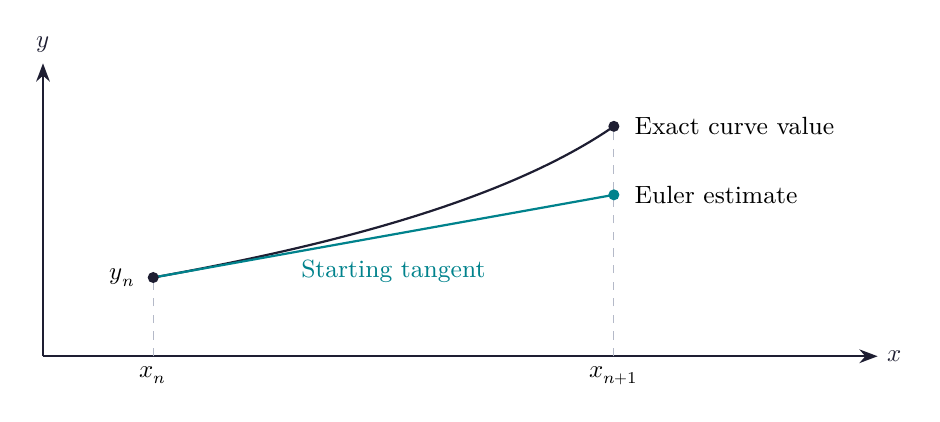
\begin{tikzpicture}[every node/.style={font=\small}]
\coordinate (a) at (1.4,1);
\coordinate (b) at (7.25,2.05);
\coordinate (c) at (7.25,2.92);
\draw[arrow] (0,0)--(10.6,0) node[right] {$x$};
\draw[arrow] (0,0)--(0,3.72) node[above] {$y$};
\draw[mgframe,dashed] (1.4,0)--(a) (7.25,0)--(c);
\draw[mydark,thick] (a) .. controls (3.4,1.36) and (5.8,1.92) .. (c);
\draw[myteal,thick] (a)--(b);
\fill[mydark] (a) circle (2pt) (c) circle (2pt);
\fill[myteal] (b) circle (2pt);
\node[left=3pt] at (a) {$y_n$};
\node[right=4pt] at (b) {Euler estimate};
\node[right=4pt] at (c) {Exact curve value};
\node[below] at (1.4,0) {$x_n$};
\node[below] at (7.25,0) {$x_{n+1}$};
\node[below,text=myteal] at (4.45,1.35) {Starting tangent};
\end{tikzpicture}\par
\end{tcolorbox}

\begin{tcolorbox}[examplebox, title={Compute two Euler steps}]
For $y'=x+y$, $y(0)=1$, use $h=0.1$.
\[
\begin{aligned}
y_1&=1+0.1(0+1)=1.10,\\
y_2&=1.10+0.1(0.1+1.10)=1.22.
\end{aligned}
\]
The exact solution is $2e^x-x-1$. At $x=0.2$ it is about $1.242806$, so the signed error (exact minus computed) is about $0.022806$.
\end{tcolorbox}

\begin{tcolorbox}[masonbox, title={Stability check}]
For $y'=\lambda y$, Euler multiplies the solution by $1+h\lambda$ in each step. For real $\lambda<0$, numerical decay requires $|1+h\lambda|<1$, or $0<h<2/|\lambda|$. An accurate order estimate applies when the step is sufficiently small.
\end{tcolorbox}

\subsection{Runge--Kutta methods}
Runge--Kutta evaluates several slopes within one step. In these formulas each $k_i$ is a slope, with the factor $h$ applied separately.

\begin{tcolorbox}[formulabox, title={Two second-order methods}]
\[
\begin{aligned}
\text{Heun:}\quad k_1&=f(x_n,y_n),\\
k_2&=f(x_n+h,y_n+hk_1),&
y_{n+1}&=y_n+\frac h2(k_1+k_2),\\[3pt]
\text{Midpoint:}\quad k_1&=f(x_n,y_n),\\
k_2&=f(x_n+h/2,y_n+hk_1/2),&
y_{n+1}&=y_n+hk_2.
\end{aligned}
\]
Both have local defect $O(h^3)$ and global error $O(h^2)$ for smooth problems.
\end{tcolorbox}

\begin{tcolorbox}[examplebox, title={One RK2 step using both forms}]
For the previous IVP, $k_1=1$ and $h=0.1$.
\begin{itemize}[leftmargin=*, itemsep=3pt, topsep=4pt]
  \item \textbf{Heun.} Predict the endpoint $(0.1,1.1)$. Its slope is $1.2$. The average gives $1+0.05(1+1.2)=1.11$.
  \item \textbf{Midpoint.} Predict $(0.05,1.05)$. Its slope is $1.10$, so the update gives $1+0.1(1.10)=1.11$.
\end{itemize}
The two different formulas happen to return the same first step on this IVP.
\end{tcolorbox}

\begin{tcolorbox}[formulabox, title={Classical fourth-order Runge--Kutta}]
\[
\begin{aligned}
k_1&=f(x_n,y_n),\\
k_2&=f(x_n+h/2,y_n+hk_1/2),\\
k_3&=f(x_n+h/2,y_n+hk_2/2),\\
k_4&=f(x_n+h,y_n+hk_3),\\
y_{n+1}&=y_n+\frac h6(k_1+2k_2+2k_3+k_4).
\end{aligned}
\]
The local defect is $O(h^5)$ and the global error is $O(h^4)$ for a smooth IVP under standard assumptions. The first midpoint slope supplies the second midpoint stage.
\end{tcolorbox}

\begin{tcolorbox}[examplebox, title={RK4 stage table on the same IVP}]
\par\vspace{5pt}
\begingroup
\setlength{\extrarowheight}{1pt}
\noindent\begin{tabularx}{\linewidth}{|B{1.7cm}|Y|Y|Y|}
\hline
\textbf{Stage} & \textbf{$x$ input} & \textbf{$y$ input} & \textbf{Slope $f=x+y$} \\ \hline
$k_1$ & $0$ & $1$ & $1$ \\ \hline
$k_2$ & $0.05$ & $1.05$ & $1.10$ \\ \hline
$k_3$ & $0.05$ & $1.055$ & $1.105$ \\ \hline
$k_4$ & $0.10$ & $1.1105$ & $1.2105$ \\ \hline
\end{tabularx}\par
\endgroup
\[
\begin{aligned}
y_1&=1+\frac{0.1}{6}(1+2.20+2.21+1.2105)\\
   &\approx1.110341667.
\end{aligned}
\]
The exact value at $0.1$ is about $1.110341836$. Keep working digits in the four slopes.
\end{tcolorbox}

\section{Predictor--Corrector Methods}
\subsection{The predict, evaluate, correct, evaluate sequence}
\begin{tcolorbox}[defbox, title={Predictor and corrector}]
A predictor uses known data to estimate the next value explicitly. A corrector uses a formula involving the slope at the new point. Use the predicted value to supply its first new-point slope.
\end{tcolorbox}

\begin{enumerate}[leftmargin=*, itemsep=3pt, topsep=4pt]
  \item \textbf{Predict.} Compute $y_{n+1}^{(p)}$ from stored values.
  \item \textbf{Evaluate.} Calculate $f_{n+1}^{(p)}=f(x_{n+1},y_{n+1}^{(p)})$.
  \item \textbf{Correct.} Compute $y_{n+1}^{(c)}$ using the predicted slope. If iteration is requested, repeat using the latest corrected slope until the change is suitably small.
  \item \textbf{Evaluate again.} Store $f(x_{n+1},y_{n+1}^{(c)})$ for future steps. The sequence is called PECE.
\end{enumerate}
A single-step pair uses Euler as predictor and $y_{n+1}^{(c)}=y_n+\tfrac h2(f_n+f_{n+1}^{(p)})$ as corrector. One correction gives Heun's method. Repeated corrections attempt to solve the implicit trapezoidal step. The multistep pairs below assume equal steps and require several accurate initial values. Use an accurate one-step method such as RK4 to generate them if needed.

\subsection{Adams--Bashforth and Adams--Moulton pair}
\begin{tcolorbox}[formulabox, title={Adams pair on a uniform grid}]
Let $f_j=f(x_j,y_j)$.
\[
\begin{aligned}
y_{n+1}^{(p)}&=y_n+\frac{h}{24}
 (55f_n-59f_{n-1}+37f_{n-2}-9f_{n-3}),\\
y_{n+1}^{(c)}&=y_n+\frac{h}{24}
 (9f_{n+1}^{(p)}+19f_n-5f_{n-1}+f_{n-2}).
\end{aligned}
\]
The predictor uses four old slopes. The fourth-order corrector uses the estimated new-point slope and the three latest old slopes.
\end{tcolorbox}

\subsection{Milne predictor and Simpson corrector}
\begin{tcolorbox}[formulabox, title={Milne--Simpson pair}]
\[
\begin{aligned}
y_{n+1}^{(p)}&=y_{n-3}+\frac{4h}{3}
 (2f_{n-2}-f_{n-1}+2f_n),\\
y_{n+1}^{(c)}&=y_{n-1}+\frac{h}{3}
 (f_{n-1}+4f_n+f_{n+1}^{(p)}).
\end{aligned}
\]
The corrector integrates the slope from $x_{n-1}$ to $x_{n+1}$ using Simpson weights. Start it from $y_{n-1}$.
\end{tcolorbox}

\begin{tcolorbox}[examplebox, title={Compare both pairs on one new node}]
For $y'=y$, $y(0)=1$ and $h=0.1$, use the exact starting values $y_j=e^{0.1j}$ for $j=0,1,2,3$. Then $f_j=y_j$. Use the formulas above to compute $y_4$.
\par\vspace{5pt}
\begingroup
\setlength{\extrarowheight}{1pt}
\noindent\begin{tabularx}{\linewidth}{|B{3.5cm}|Y|Y|}
\hline
\textbf{Pair} & \textbf{Prediction} & \textbf{After one correction} \\ \hline
Adams & $1.491820456$ & $1.491824885$ \\ \hline
Milne--Simpson & $1.491820892$ & $1.491824721$ \\ \hline
\end{tabularx}\par
\endgroup
For Milne--Simpson substitute $y_2=f_2=1.221402758$, $f_3=1.349858808$ and $f_4^{(p)}=1.491820892$ into $y_2+(0.1/3)(f_2+4f_3+f_4^{(p)})$. The exact value $e^{0.4}$ is about $1.491824698$. All table entries are rounded after computation.
\end{tcolorbox}

\section{Finite Difference Method for Boundary Values}
\subsection{Centred derivatives and grid equations}
Use $x_i=a+ih$ and write $Y_i$ for the computed value. Subtract Taylor expansions at $x_i\pm h$ to approximate the first derivative. Add them to approximate the second derivative.
\begin{tcolorbox}[formulabox, title={Three-point centred formulas}]
\[
\begin{aligned}
y'(x_i)&=\frac{y(x_{i+1})-y(x_{i-1})}{2h}+O(h^2),\\
y''(x_i)&=\frac{y(x_{i-1})-2y(x_i)+y(x_{i+1})}{h^2}+O(h^2).
\end{aligned}
\]
Odd powers cancel in the sum and even powers cancel in the difference. These are truncation errors of the derivative formulas for smooth solutions.
\end{tcolorbox}

\begin{enumerate}[leftmargin=*, itemsep=3pt, topsep=4pt]
  \item \textbf{Discretise each interior row.} For $y''+p(x)y'+q(x)y=r(x)$, multiply by $h^2$ after replacing the derivatives:
 \[
 (1-hp_i/2)Y_{i-1}+(h^2q_i-2)Y_i+
       (1+hp_i/2)Y_{i+1}=h^2r_i.
 \]
  \item \textbf{Insert the boundary data.} Substitute $Y_0=\alpha$ and $Y_N=\beta$. Move their contributions to the right-hand side of the first and last interior rows.
  \item \textbf{Solve and check.} Each row uses three adjacent grid values, giving a tridiagonal matrix. Check the residual of the discrete equations and both boundary values.
\end{enumerate}
\begin{tcolorbox}[examplebox, title={Solve a boundary-value problem on a five-node grid}]
Take $y''=-2$ on $[0,1]$, $y(0)=y(1)=0$, and $h=1/4$. The interior equations, multiplied by $-h^2$, are
\[
\left[\begin{array}{rrr|r}
 2&-1&0&1/8\\
 -1&2&-1&1/8\\
 0&-1&2&1/8
\end{array}\right].
\]
By symmetry $Y_1=Y_3=a$ and $Y_2=b$, so $2a-b=1/8$ and $2b-2a=1/8$. The second equation gives $b=a+1/16$. Substitute into the first to obtain $a=3/16$ and $b=1/4$. The exact solution is $y=x(1-x)$. The values match at the nodes because the centred second difference is exact for a quadratic.
\end{tcolorbox}

\newpage
\begin{center}
  {\large\bfseries\color{myred} Quick Revision --- Module 3}\\[3pt]
  {\small\color{mydark} Numerical Solutions of Ordinary Differential Equations $|$ BS-M401}
\end{center}
\noindent{\color{myred}\rule{\linewidth}{1.2pt}}\par\vspace{4pt}

\begin{tcolorbox}[formulabox, title={Key Concepts at a Glance}]
\renewcommand{\arraystretch}{1.35}
\noindent\begin{tabularx}{\linewidth}{B{4.5cm}Y}
Euler & $y_{n+1}=y_n+hf_n$. Global order one. \\[3pt]
RK2 & Two slopes per step. Heun averages endpoint slopes and midpoint uses a midpoint estimate. \\[3pt]
RK4 & Weights $1,2,2,1$ on the slopes, with multiplier $h/6$. \\[3pt]
Predictor--corrector & Predict, evaluate, correct, then evaluate again. \\[3pt]
Centred second difference & $(Y_{i-1}-2Y_i+Y_{i+1})/h^2$. \\[3pt]
\end{tabularx}\par
\end{tcolorbox}

\begin{tcolorbox}[defbox, title={One-Line Definitions}]
\begin{itemize}[leftmargin=*, itemsep=3pt, topsep=4pt]
  \item \textbf{IVP.} Known conditions at the starting point.
  \item \textbf{BVP.} Conditions specified at different points.
  \item \textbf{Local defect.} Error from one update started with exact data.
  \item \textbf{Stencil.} Grid locations used to approximate a derivative.
\end{itemize}
\end{tcolorbox}

\begin{tcolorbox}[exambox, title={Frequently Asked / Viva Questions}]
\begin{enumerate}[topsep=0pt, label=\textbf{Q\arabic*.}, itemsep=5pt, leftmargin=*]
  \item \Q{How is Euler derived?}
    Keep the constant and first-derivative terms in the Taylor expansion.
  \item \Q{What is Euler's global order?}
    First order for a sufficiently smooth, well-posed IVP.
  \item \Q{What distinguishes the two midpoint stages of classical RK4?}
    The first uses the starting slope and the second uses the first midpoint slope.
  \item \Q{How many slopes does classical RK4 evaluate per step?}
    Four.
  \item \Q{What is the one-step local defect of RK4?}
    $O(h^5)$ for a sufficiently smooth problem.
  \item \Q{Why do multistep methods need starting values?}
    Their formulas use several previously computed slopes.
  \item \Q{How is the first slope used in the corrector found?}
    Evaluate the ODE at the predicted new-point value.
  \item \Q{Where does Milne's Simpson corrector start?}
    At $y_{n-1}$. Its integration panel spans $x_{n-1}$ to $x_{n+1}$.
  \item \Q{Why does the three-point stencil yield a tridiagonal system?}
    Each row relates the current node to its two neighbours.
  \item \Q{How are prescribed endpoints handled?}
    Substitute them into the outer interior rows and move the known terms to the right-hand side.
  \item \Q{Does a second-order stencil ensure a good answer on any grid?}
    Solution accuracy also depends on the step size, smoothness and stability of the discretisation.
\end{enumerate}
\end{tcolorbox}

\begin{tcolorbox}[tikzbox, title={Summary Comparison}]
\par\vspace{5pt}
\begingroup
\setlength{\extrarowheight}{1pt}
\noindent\begin{tabularx}{\linewidth}{|B{3.45cm}|Y|Y|}
\hline
\textbf{Method} & \textbf{Typical use} & \textbf{Main check} \\ \hline
Euler & Quick first-order IVP estimate. & Check accuracy and stability at the selected step. \\ \hline
Runge--Kutta & Accurate one-step IVP computation. & Keep stage locations and the slope convention consistent. \\ \hline
Predictor--corrector & Continue a uniformly spaced IVP solution. & Use accurate starting values and correct slope indices. \\ \hline
Finite difference & Assemble a BVP system. & Insert both endpoint conditions. \\ \hline
\end{tabularx}\par
\endgroup
\end{tcolorbox}

\end{document}
